% -*- TeX -*-
\documentclass{beamer}

\title{Crustal Deformation Modeling Tutorial}
\subtitle{Running PyLith in Parallel}
\author{Brad Aagaard \\
  Matthew Knepley \\
  Charles Williams}
\institute{
\includegraphics[scale=0.4]{../../logos/cig_blackfg}}
\date{June 28, 2013}


% ---------------------------------------------------- CUSTOMIZATION
\renewcommand{\thispdfpagelabel}[1]{}
\newcommand{\important}[1]{{\color{red}#1}}
\usetheme{CIG}

% ========================================================= DOCUMENT
\begin{document}

% ------------------------------------------------------------ SLIDE
\maketitle

% ------------------------------------------------------------ SLIDE
\logo{
\includegraphics[height=4.5ex]{../../logos/cig_blackfg}}

% ========================================================== SECTION
\section{Introduction}

% ------------------------------------------------------------ SLIDE
\begin{frame}
  \frametitle{Concepts Covered in this Session}
  \summary{}

  \begin{itemize}
  \item Running PyLith in parallel
    \begin{itemize}
    \item Desktop or laptop with multiple processors and/or cores
    \item Cluster with multiple compute nodes
    \end{itemize}
  \item Optimizing PyLith performance
  \item Building PyLith from source
  \item Using PyLith with a queue system
  \item PyLith parallel performance
  \end{itemize}

\end{frame}


% ========================================================== SECTION
\section{Running in Parallel}
\subsection{Overview}

% ------------------------------------------------------------ SLIDE
\begin{frame}
  \frametitle{Running PyLith in Parallel}
  \summary{}

  \begin{itemize}
  \item Laptop/Desktop
    \begin{itemize}
    \item Reduce runtime (distribute floating point operations)
    \item Available with binary {\tt --nodes=NUMCORES}
    \end{itemize}
  \item Cluster
    \begin{itemize}
    \item Reduce runtime (distribute floating point operations)
    \item Run larger problems (distribute memory usage)
    \item Must build from source for proper configuration
    \item Requires additional parameters for batch submission
    \end{itemize}
  \end{itemize}

\end{frame}


% ------------------------------------------------------------ SLIDE
\begin{frame}
  \frametitle{How PyLith Runs in Parallel}
  \summary{Single Program, Multiple Data (SPMD) Parallel Processing}

  \begin{enumerate}
  \item Process 0
    \begin{enumerate}
    \item Read in mesh
    \item Add cohesive cells by adjusting the mesh topology
    \item Partition mesh and determine vertices shared by multiple
      processes
    \item Distribute relevant portion of mesh to each process
    \end{enumerate}
  \item All processes
    \begin{enumerate}
    \item OPTIONAL Each processor refines its part of the mesh
    \item Each processor solves equations on its portion of the mesh,
      exchanging information as necessary with its neighbors
    \end{enumerate}
  \end{enumerate}

\end{frame}


% ------------------------------------------------------------ SLIDE
\begin{frame}
  \frametitle{Optimizing PyLith Performance}
  \summary{Efficiency depends on choice of parameters and hardware}

  \begin{itemize}
  \item Output
    \begin{description}
    \item[VTK] Inefficient: each process sends it data to process 0
      for writing
    \item[HDF5] Efficient: each process writes its own data in binary
    \end{description}
  \item Solver performance
    \begin{description}
    \item[Quasi-static] Field split with algebraic multigrid generally
      scales better than Additive Schwarz
    \item[Dynamic] Trivial solve scales extremely well
    \end{description}
  \item Overall performance
    \begin{itemize}
    \item Speed of memory and connection b/t memory and CPU is more
      important than CPU speed
    \item Marginal speed improvement if you compile source for your hardware
    \end{itemize}
  \end{itemize}

\end{frame}


% ========================================================== SECTION
\subsection{Desktop}

% ------------------------------------------------------------ SLIDE
\begin{frame}
  \frametitle{Running PyLith in Parallel on a Desktop}
  \summary{Reduce runtime using multiple processors and/or cores}

  \vfill
  Add number of processes (usually number of cores) as argument:\\
  {\tt pylith \important{--nodes=NUMCORES}} 
  \vfill

  \begin{itemize}
  \item PyLith binary
    \begin{itemize}
    \item Allows interprocess communication only within
      a single computer
    \item Works with laptops, desktops, and a single compute node
    \end{itemize}
  \item Building PyLith from source
    \begin{itemize}
    \item Permits optimizing code for your hardware; may provide modest
      performance gains
    \end{itemize}
  \end{itemize}

\end{frame}


% ========================================================== SECTION
\subsection{Cluster}

% ------------------------------------------------------------ SLIDE
\begin{frame}
  \frametitle{Running PyLith on a Cluster}
  \summary{For large quasi-static and 3-D dynamic simulations}

  \begin{itemize}
  \item Differences from usage on a desktop machine
    \begin{itemize}
    \item Usually requires additional parameters for batch
      queue system
    \item {\bf Strongly} recommend using {\tt\important{DataWriterHDF5Ext*}} for output
      \begin{itemize}
      \item Parallel output via shared or parallel file system
      \item More failsafe than regular HDF5 output ({\tt
          DataWriterHDF5*})
      \end{itemize}
    \item Stdout and stderr are written to a log file or files
    \end{itemize}
  \item Consult your system administrator on MPI parameters
  \item Read getting started guides provided by computing centers
    \begin{itemize}
    \item What compiler suites and MPI versions are available?
    \item What filesystems are available? Which support parallel I/O?
    \end{itemize}
  \end{itemize}

\end{frame}


% ------------------------------------------------------------ SLIDE
\begin{frame}
  \frametitle{Hints for Running PyLith on a Cluster}
  \summary{How many compute nodes and cores should I use?}

  \begin{itemize}
  \item General
    \begin{itemize}
    \item If you have N compute nodes and want to run J jobs, use N/J
      compute nodes
    \item Use the maximum number allowable by the queue with the
      shortest wait
    \item Don't overload a compute node (memory use exceeds that
      available)
    \item Don't overload fileservers
    \end{itemize}
  \item Quasi-static problems
    \begin{itemize}
    \item Memory use and runtime depends on the solver parameters
    \item Memory use is often dominated by the sparse matrix
    \item Different bulk rheologies use different amounts of memory
    \end{itemize}
  \item Dynamic problems
    \begin{itemize}
    \item Don't overload compute nodes
    \item Spontaneous rupture uses more memory than prescribed slip
    \end{itemize}
  \end{itemize}

\end{frame}


% ========================================================== SECTION
\section{Parallel Performance}
\subsection{}

% ------------------------------------------------------------ SLIDE
\begin{frame}
  \frametitle{PyLith Parallel Performance Test}
  \summary{Static solution of prescribed slip on multiple faults}

  \begin{center}
    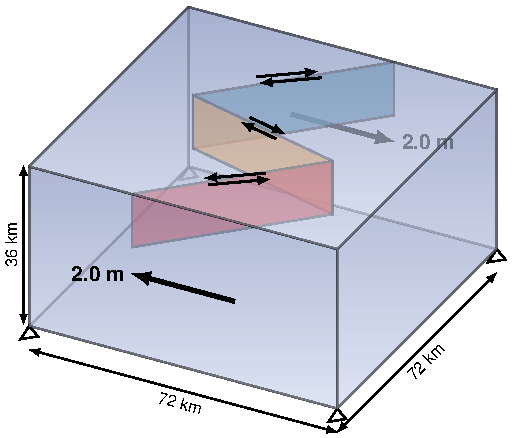
\includegraphics[height=7.0cm]{figs/solvertest_geometry}
  \end{center}

\end{frame}


% ========================================================== SECTION
\subsection{Preconditioners}

% ------------------------------------------------------------ SLIDE
\begin{frame}
  \frametitle{PyLith Parallel Performance Test}
  \summary{Field split and AMG with custom fault preconditioner performs best}

  \begin{center}
    Number of Iterations in Linear Solve\\[4pt]
\begin{tabular}{lcrrr}
  \hline
  Preconditioner & Cell & \multicolumn{3}{c}{Problem Size} \\
     &      & S1 & S2 & S4 \\
  \hline
  ASM
    & Tet4 & 184 & 217 & 270 \\
    & Hex8 & 143 & 179 & 221 \\
  Schur (full)
    & Tet4 & 82 & 84 & 109 \\
    & Hex8 & 54 & 60 & 61 \\
  Schur (upper)
    & Tet4 & 79 & 78 & 87 \\
    & Hex8 & 53 & 59 & 57 \\
  FieldSplit (add)
    & Tet4 & 241 & 587 & 585 \\
    & Hex8 & 159 & 193 & 192 \\
  FieldSplit (mult)
    & Tet4 & 284 & 324 & 383 \\
    & Hex8 & 165 & 177 & 194 \\
  \important{FieldSplit (mult,custom)}
    & Tet4 & 42 & 48 & 51 \\
    & Hex8 & 35 & 39 & 43 \\
\hline
\end{tabular}
  \end{center}
  
\end{frame}


% ========================================================== SECTION
\subsection{Parallel Scaling}

% ------------------------------------------------------------ SLIDE
\begin{frame}
  \frametitle{PyLith Parallel Performance Test}
  \summary{Weak scaling of field split w/AMG and custom fault preconditioner}

  \begin{center}
    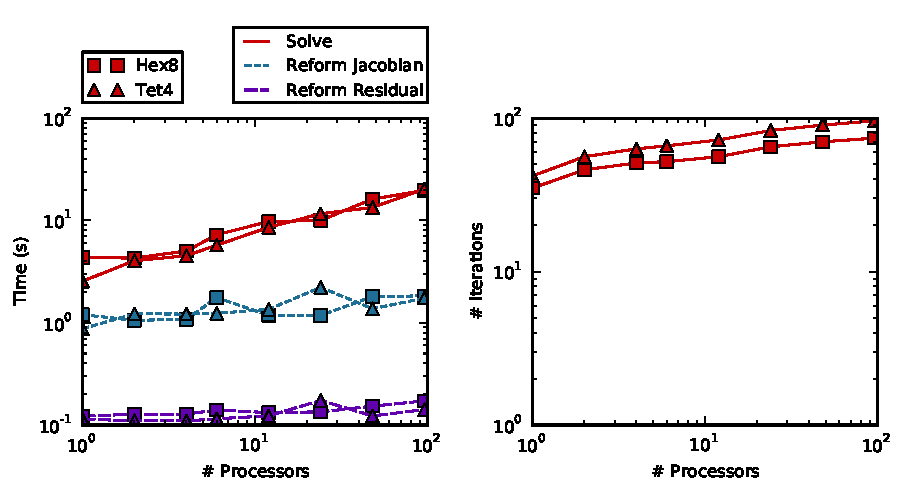
\includegraphics[width=11.0cm]{figs/solvertest_scaling}
  \end{center}
  
\end{frame}


% ------------------------------------------------------------ SLIDE
\begin{frame}[fragile]
  \frametitle{Dissecting PETSc Log Summary I}
  \summary{Where are the bottlenecks?}

  \begin{minipage}[b]{5cm}
  \begin{center}
  Quasi-Static Simulation \\
  Savage-Prescott Benchmark \\
{\tiny
\begin{verbatim}
Summary of Stages:   ----- Time ------
                        Avg     %Total
 0:      Main Stage: 5.7474e+00   0.2%
 1:         Meshing: 1.6935e+01   0.6%
 2:           Setup: 1.4908e+01   0.5%
 3: Reform Jacobian: 5.2058e+00   0.2%
 4: Reform Residual: 1.4038e+02   5.1%
 5:           Solve: 2.3698e+03  85.8%
 6:         Prestep: 1.2892e+01   0.5%
 7:            Step: 6.8484e+01   2.5%
 8:        Poststep: 1.2611e+02   4.6%
 9:        Finalize: 4.6684e-01   0.0%
\end{verbatim}}
\end{center}
\end{minipage}
\hfill
  \begin{minipage}[b]{5cm}
  \begin{center}
  Dynamic Simulation\\
  SCEC Dynamic Rupture \\
  Benchmark TPV102
{\tiny
\begin{verbatim}
Summary of Stages:   ----- Time ------
                        Avg     %Total
 0:      Main Stage: 3.4975e+00   0.1%
 1:         Meshing: 1.5496e+02   3.6%
 2:           Setup: 8.6702e+01   2.0%
 3: Reform Jacobian: 3.5730e+00   0.1%
 4: Reform Residual: 2.5464e+03  59.6%

 6:         Prestep: 3.1002e+00   0.1%
 7:            Step: 1.2559e+03  29.4%
 8:        Poststep: 2.1854e+02   5.1%
 9:        Finalize: 1.0401e+00   0.0%
\end{verbatim}}
\end{center}
\end{minipage}

\end{frame}


% ------------------------------------------------------------ SLIDE
\begin{frame}
  \frametitle{Dissecting PETSc Log Summary II}
  \summary{Identify memory bandwidth saturation and communication bottlenecks}

  \begin{center}
{\tiny
\begin{tabular}{lrrrl}
  \hline
  Event & \# Cores & Load Imbalance & MFlops/s & Comments \\
  \hline
VecMDot &    1 & 1.0 &   2007 \\
     &    2 & 1.1 &   3809 \\
     &    4 & 1.1 &   5431 \\
     &    6 & 1.1 &   5967 & Memory bandwidth saturation \\
     &   12 & 1.2 &   5714 \\
     &   24 & 1.2 &  11784 & Multiple compute nodes, scaling returns \\
     &   48 & 1.2 &  20958 \\
     &   96 & 1.3 &  17976 & Inter-compute node saturation? \\
  \hline
VecAXPY &    1 & 1.0 &   1629 \\
     &    2 & 1.1 &   3694 \\
     &    4 & 1.1 &   5969 \\
     &    6 & 1.1 &   6028 & Memory bandwidth saturation \\
     &   12 & 1.2 &   5055 \\
     &   24 & 1.2 &  10071 & Multiple compute nodes, scaling returns \\
     &   48 & 1.2 &  18761 \\
     &   96 & 1.3 &  33676 \\
  \hline
VecMAXPY &    1 & 1.0 &   1819 \\
     &    2 & 1.1 &   3415 \\
     &    4 & 1.1 &   5200 \\
     &    6 & 1.1 &   5860 & Memory bandwidth saturation \\
     &   12 & 1.2 &   6051 \\
     &   24 & 1.2 &  12063 & Multiple compute nodes, scaling returns\\
     &   48 & 1.2 &  23072 \\
     &   96 & 1.3 &  28461 \\
  \hline
\end{tabular}}
\end{center}

\end{frame}


% ------------------------------------------------------------ SLIDE
\begin{frame}
  \frametitle{PyLith v1.9 versus v2.0}
  \summary{Under-the-hood improvements fix some parallel scaling issues}

  \begin{itemize}
  \item PyLith v1.9
    \begin{itemize}
    \item Reading in mesh by single process limits size of calculation
    \item Dynamic problems with $>$50M cells (hex or tet)
    \item Memory imbalance of up to 10x for large problems with faults
    \end{itemize}
  \item PyLith v2.0
    \begin{itemize}
    \item Reading in mesh by single process limits size of calculation
    \item Improved mesh data structures reduce memory use
    \item Expect memory balancing to be very good
    \item Expect to be able to run problems with O(10$^8$) cells
    \end{itemize}
  \end{itemize}

\end{frame}

% ========================================================== SECTION
\section{Running on a Cluster}
\subsection{Building from Source}

% ------------------------------------------------------------ SLIDE
\begin{frame}
  \frametitle{Building PyLith from Source}
  \summary{Required for PyLith to use multiple compute nodes on a cluster}

  \begin{center}
    {\bf\important{Use the PyLith installer utility!!!}} \\
    {\tt pylith-installer-1.9.0-0.tgz}
  \end{center}

  \begin{itemize}
  \item Downloads, configures, and builds PyLith and dependencies
  \item User selects which dependencies are needed and installer will
    do some minimal checks
  \item Insures versions, configuration, and builds are consistent
    PyLith requirements
  \item See INSTALL file in installer tarball for instructions
  \end{itemize}

\end{frame}


% ========================================================== SECTION
\subsection{Using a Queue System}

% ------------------------------------------------------------ SLIDE
\begin{frame}
  \frametitle{Submitting Jobs to PBS Queue System}
  \summary{PBS is one of the most common batch queue systems}

  \begin{itemize}
    \item PyLith uses Pyre to submit jobs directly to PBS
    \begin{enumerate}
    \item Perform minimal validation of the simulation parameters
    \item Create a shell script to submit job
    \item Submit job
    \end{enumerate}
  \item Assumes you have already setup running jobs on the cluster
  \end{itemize}
  
\end{frame}


% ------------------------------------------------------------ SLIDE
\begin{frame}[fragile]
  \frametitle{Submitting Jobs to PBS Queue System}
  \summary{}

  Put parameters common to all jobs in {\tt \$HOME/.pyre/pylithapp/pylithapp.cfg}

{\small
\begin{verbatim}
[pylithapp]
scheduler = pbs

[pylithapp.pbs]
# Shell used for job script submitted to batch system
shell = /bin/bash
# Command line arguments in qsub command
# -V = Use current environment variables in batch job
# -m bea = Send email when job begins, ends, or aborts
qsub-options = -V -m bea -M johndoe@university.edu

[pylithapp.launcher]
command = mpirun -np ${nodes} -machinefile ${PBS_NODEFILE}
  \end{verbatim}}
\end{frame}


% ------------------------------------------------------------ SLIDE
\begin{frame}[fragile]
  \frametitle{Submitting Jobs to PBS Queue System}
  \summary{}

  Pass job specific parameters via the command line

  \begin{description}
  \item[{\tt--nodes=NPROCS}] Total number of processes
  \item[{\tt--scheduler.ppn=PPN}] Number of processes per compute node
  \item[{\tt --job.name=NAME}] Name of job
  \item[{\tt --job.stdout=LOG\_FILE}] File where stdout is written
  \end{description}

  \vfill
  {\tt NPROCS} $=$ {\tt NCOMPUTENODES} $\times$ {\tt PPN}
  \vfill

\end{frame}

% ------------------------------------------------------------ SLIDE
\begin{frame}[fragile]
  \frametitle{Debug Launching Parallel Jobs on Queue System}
  \summary{Use command line help features to see commands being processed}

  \begin{itemize}
  \item See default and set parameters
    \begin{description}
    \item[{\tt--COMPONENT.help-properties}] See properties and their values
    \item[{\tt--COMPONENT.help-components}] See subcomponents
    \item[{\tt pylithinfo PYLITH\_ARGS}] Dumps all parameters to {\tt pylith\_parameters.txt}
    \end{description}
  \item Submitting to the queue (scheduler)
    \begin{description}
    \item[{\tt --scheduler.help}] See list of properties/components available
    \item[{\tt --scheduler.dry}] Dump script for batch submission to
      stdout
    \end{description}
  \item Launching job on compute nodes (launcher)
    \begin{description}
    \item[{\tt --launcher.help}] Total number of processes
    \item[{\tt --launcher.dry}] Dump launching command to stdout
    \end{description}
  \end{itemize}
  
  
\end{frame}

% ======================================================================
\end{document}


% End of file
